\documentclass[12pt]{article}%
\usepackage[paper=portrait,pagesize]{typearea}
\usepackage{amssymb}
\usepackage{amsfonts}
\usepackage{amsmath}
\usepackage{hyperref}
\usepackage{lscape}
\usepackage{comment}
\usepackage[flushleft]{threeparttable}
\usepackage{float}
\usepackage[nohead]{geometry}
\usepackage[singlespacing]{setspace}
\usepackage[paper=portrait,pagesize]{typearea}
\usepackage{amssymb}
\usepackage{amsfonts}
\usepackage{multicol}
\usepackage{amsmath}
\usepackage{hyperref}
\usepackage[nameinlink,noabbrev]{cleveref}
\usepackage{lscape}
\usepackage{float}
\usepackage[nohead]{geometry}
\usepackage[singlespacing]{setspace}
\usepackage[bottom]{footmisc}
\usepackage{indentfirst}
\usepackage{endnotes}
\usepackage{graphicx}%
\usepackage{afterpage}
\usepackage{subfig}
\usepackage{rotating}
\newcommand\tab[1][1cm]{\hspace*{#1}}
\DeclareMathOperator*{\Max}{Max}
\newcommand\numberthis{\addtocounter{equation}{1}\tag{\theequation}}
\def\dotfill#1{\cleaders\hbox to #1{.}\hfill}
\newcommand\dotline[2][.5em]{\leavevmode\hbox to #2{\dotfill{#1}\hfil}}
%\usepackage[backend=biber,style=alphabetic,sorting=ynt]{biblatex}
%\addbibresource{bibliocopulas.bib}
\usepackage[round,sort,comma,authoryear]{natbib}
\setcounter{MaxMatrixCols}{30}
\newtheorem{theorem}{Theorem}
\newtheorem{acknowledgement}{Acknowledgement}
\newtheorem{algorithm}[theorem]{Algorithm}
\newtheorem{axiom}[theorem]{Axiom}
\newtheorem{case}[theorem]{Case}
\newtheorem{claim}[theorem]{Claim}
\newtheorem{conclusion}[theorem]{Conclusion}
\newtheorem{condition}[theorem]{Condition}
\newtheorem{conjecture}[theorem]{Conjecture}
\newtheorem{corollary}[theorem]{Corollary}
\newtheorem{criterion}[theorem]{Criterion}
\newtheorem{definition}[theorem]{Definition}
\newtheorem{example}[theorem]{Example}
\newtheorem{exercise}[theorem]{Exercise}
\newtheorem{lemma}[theorem]{Lemma}
\newtheorem{notation}[theorem]{Notation}
\newtheorem{problem}[theorem]{Problem}
\newtheorem{proposition}{Proposition}
\newtheorem{remark}[theorem]{Remark}
\newtheorem{solution}[theorem]{Solution}
\newtheorem{summary}[theorem]{Summary}
\newenvironment{proof}[1][Proof]{\noindent\textbf{#1.} }{\ \rule{0.5em}{0.5em}}
\newcommand{\pd}[2]{\frac{\partial#1}{\partial#2}}
\makeatletter
\def\@biblabel#1{\hspace*{-\labelsep}}
\makeatother
\geometry{left=1in,right=1in,top=1.00in,bottom=1.0in}
%\renewcommand*\abstractname{Summary}

\begin{document}

\title{Fall 2019 - ECON 634 - Advance Macroeconomics - Problem Set 2}
\author{Elisa Taveras Pena\footnote{E-mail address: \href{mailto:etavera2@binghamton.edu}{etavera2@binghamton.edu}  }\\
Binghamton University}
\maketitle

\sloppy%avoids the breakage of words at the end of lines, by adjusting spaces between words inside the lines

\onehalfspacing

\begin{enumerate}
	\item 
	
	Since the Resource constraint (Social Planner Problem) is $c_t=A_tk_{t}^\alpha+(1-\delta)k_{t}-k_{t+1}$ we can write the budget constraint  in recursive form as  $c=Ak^\alpha+(1-\delta)k-k'$ 
	
	\tab \textbf{ $\bullet$ State variable}: $k,A$ 
	
	\tab \textbf{ $\bullet$ Control variable}: $k'$
	
	
	
	Therefore, the Bellman equation:
	
	\begin{align*}
	&V(k,A)=\Max_{k'} \left\lbrace \frac{\left( Ak^\alpha+(1-\delta)k-k'\right) ^{1-\sigma}}{1-\sigma}+ \beta \sum_{A' \in A} \Pi(A'|A)V(k',A')\right\rbrace 
	& \notag \\
	&\text{subject to} \notag \\
	& \tab c \in [0,f(k)] \numberthis\\
	& \tab k' \in [0,f(k)] \ \numberthis\\
	\end{align*} 
	
	\item Using the VFI, the Graphs are like follows:
	
	\begin{center}
		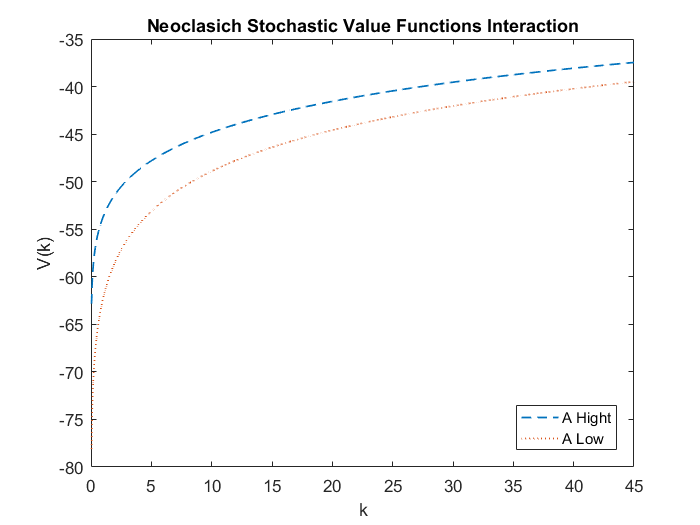
\includegraphics[width=1\linewidth]{VF}
	\end{center}
	
	
	As we can see, both are increasing and concave functions. 
	
	\item  The Policy function over $k$ looks as follows:
	
	\begin{center}
		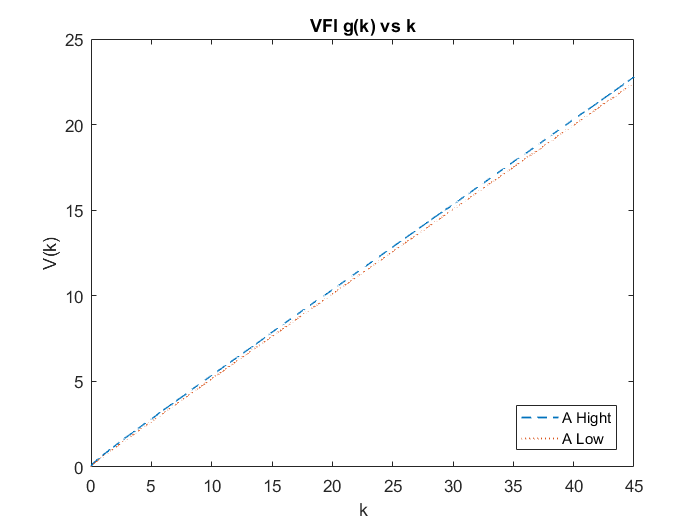
\includegraphics[width=1\linewidth]{g_k}
	\end{center}
	
	
	The Saving over $k$ looks as follows:

	
	\item In the Long run, for the NGM, 
	
\end{enumerate}

\strut

\onehalfspacing

\end{document}
